\section{Einführung}
\paragraph{Logical- und Visual-Tree}
Der \textbf{Logical Tree} enstpricht der Struktur der XAML Elemente. Es beschreibt Beziehungen zwischen verschiedenen Elementen des UIs. Der \textbf{Visual Tree} entspricht der grafischen Repräsentation und beinhaltet alle dargestellten Elemente gemäss der Vorlage jedes Controls. \\
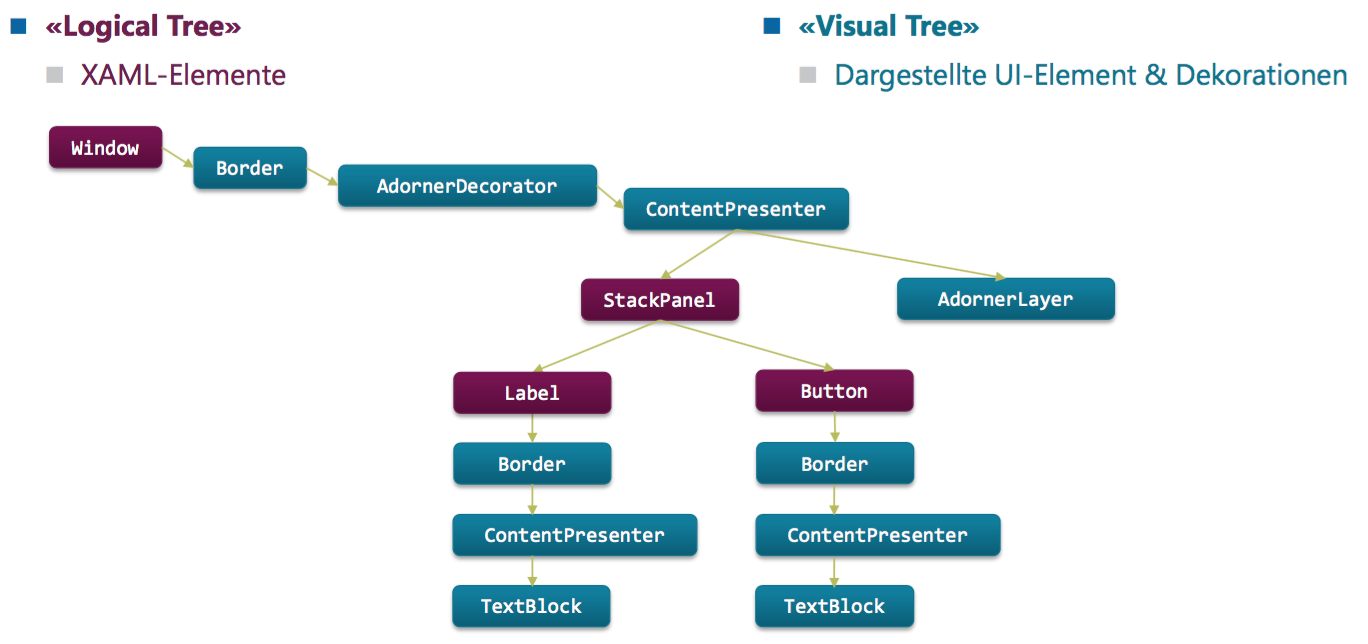
\includegraphics[scale=0.27]{LogicalVisual.png}
Der Logical-Tree entspricht der Strukutr der XAML-Elemente. Sie beschreibt die Beziehungen zwischen verschiedenen Elementen des UI. Es ist Zuständig für:
\begin{itemize}
    \item Dependency Properties erben
    \item Dynamische Ressourcen-Referenzen auflösen
    \item Elementnamen für Datenbindung nachschlagen
    \item Routed Events weiterleiten
\end{itemize}
Der Visual-Tree entspricht der grafischen Repräsentation und beinhaltet alle dargestellten Elemente gemäss der Vorlage jedes Controls. Es ist Zuständig für:
\begin{itemize}
    \item Visuelle Darstellung
    \item Vererben der Transparenzeinstellungen
    \item Vererben von Transformationen
    \item Vererben der IsEnabled-Property
    \item Hit-Testing
\end{itemize}
\paragraph{Property Syntax} XAML verwendet die Property Syntax wohingegen HTML beispielsweise Attribute Syntax verwendet.
\section{Layout und Controls}
\begin{lstlisting}[language=xml]
<Button Height="50" Width="200" Content="Watch Now" />

<Button Width="120" Height="50">
  <Button.Content>Watch Now</Button.Content>
</Button>

<Button Width="120" Height="50">
  <Button.Content>
    <StackPanel>
     <TextBlock Text="Watch Now" FontSize="20" />
     <TextBlock Text="Duration: 50m" FontSize="12" 
        Foreground="#888888" />
    </StackPanel>
  </Button.Content>
</Button> 
\end{lstlisting}

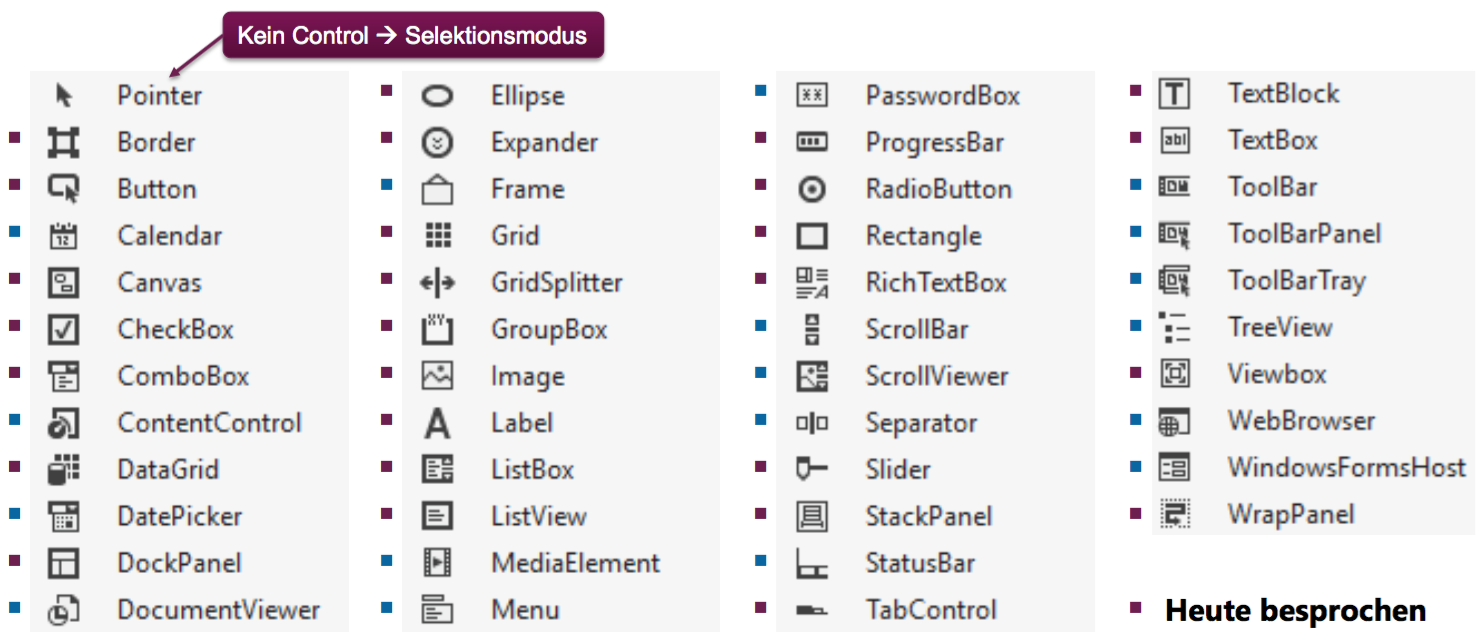
\includegraphics[scale=0.25]{ControlsOverview.png}
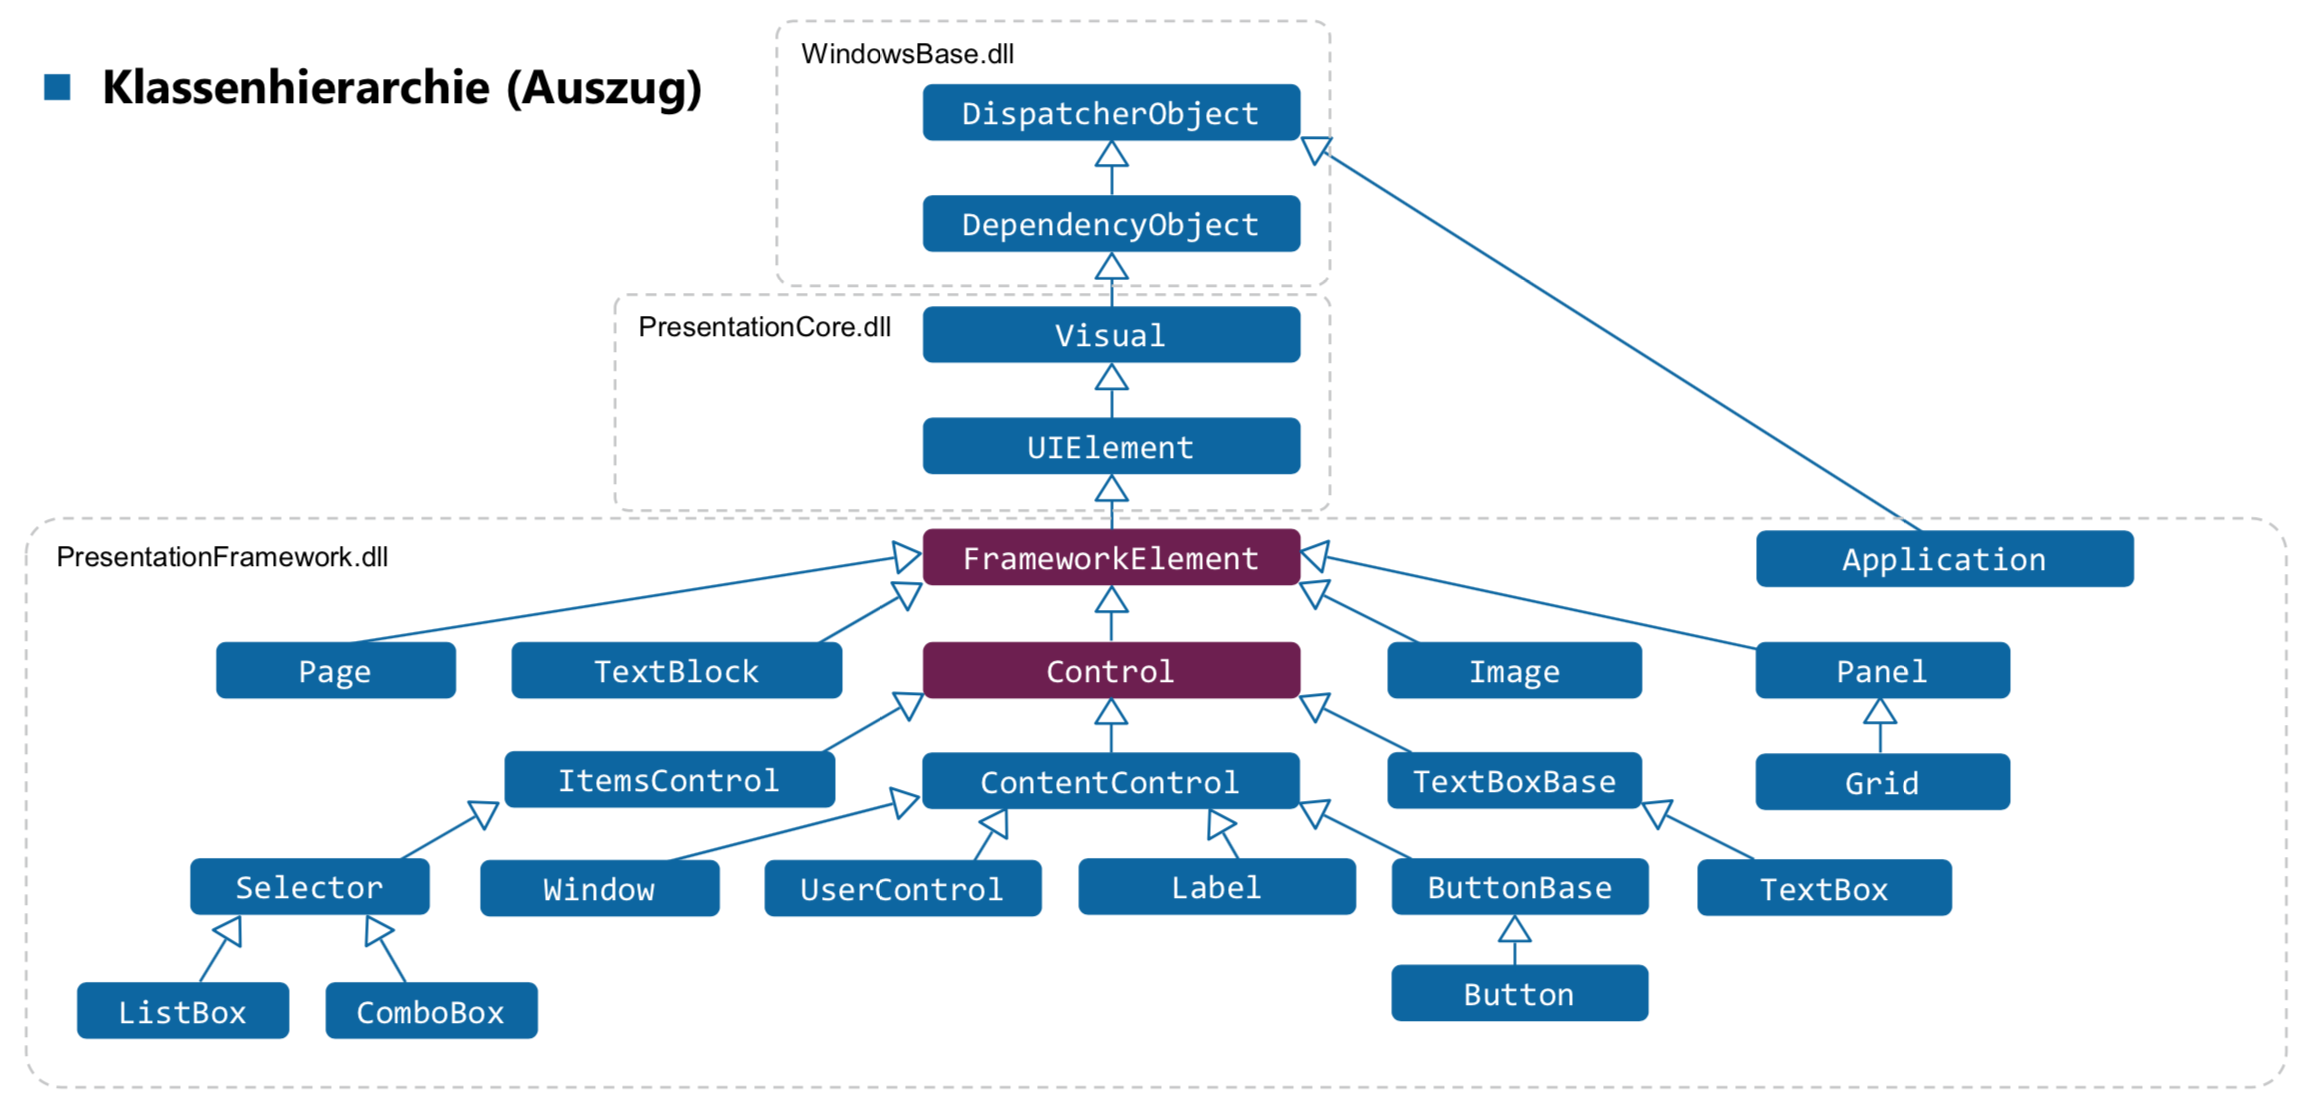
\includegraphics[scale=0.30]{Klassenhierarchie.png}
\paragraph{Grössenangaben} Zur Manipulation von Width und Height Attributen (\code{System.Windows.FrameworkElement}) kann man fixe Grössenangaben verwenden, diese werden als \code{double} Werte geschrieben. Wenn kein Kennzeichner angegeben ist (nur eine Zahl), wird automatisch \textit{Device Independent Pixel} verwendet $\left(\frac{1}{96}''\right)$. Qualfizierte Grössenangaben sind:
\begin{itemize}
\item \textbf{px} Device Independent Pixels $\left(1\text{px} = \frac{1}{96}''\right)$
\item \textbf{in} Inches (Zoll) $1\text{in} = 96\text{px}$
\item \textbf{cm} $1\text{cm} = \frac{96}{2.54}\text{px}$
\item \textbf{pt} Points $1\text{pt} = \frac{1}{72}'' = \frac{96}{72}\text{px}$
\end{itemize}
Zusätzlich kann man noch \code{MinWidth} und \code{MaxWidth} definieren. Bei Platzproblemen wird zuerst MinWidth, dann MaxWidth und dann Width evaluiert. Das Read-only Property \code{ActualWidth} kann verwendet werden um die Fenstergrösse während der Laufzeit abzufragen. 
\paragraph{Ausrichtung} HorizontalAlignment und VerticalAlignment Attribute manipulieren die Ausrichtung innerhalb des Containers. Es gibt auch HorizontalContentAlignment und VerticalContentAlignment für Inhaltsaurichtung beispielsweise für TextBox. Valide Werte sind: Left, Center, Right und Stretch für Horizontal bzw. Top, Center, Bottom und Stretch für Vertical. Stretch füllt jeweils die komplette Verfügbare Achse. \textbf{Stretch hat jeweils eine tiefere Priorität als fixe Width/Height-Angaben!}
\paragraph{Ränder \& Rahmen} Um Rahmengrössen anzupassen gibt es Margin, Padding, BorderThickness und CornerRadius. Für die ersten 3 sind folgende Werte zulässig
\begin{itemize}
\item \textbf{l,t,r,b}
\item \textbf{l,t} Left=Right, Top=Bottom
\item \textbf{x} Auf allen Seiten gleich viel Abstand
\end{itemize}
Bei Corner Radius gibt es nur eine zulässige Definition:
\begin{itemize}
\item TopLeft, TopRight, BottomRight, BottomLeft
\end{itemize}
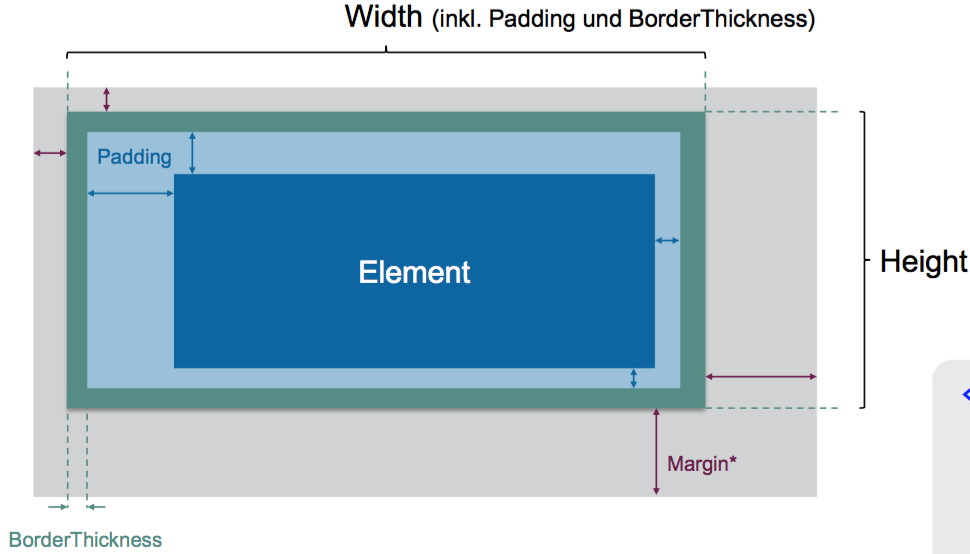
\includegraphics[scale=0.35]{Rahmen.png}
Auf jedes \textbf{UIElement} kann man noch \code{IsEnabled}, \code{SnapsToDevicePixels} (Rundet Pixelangaben auf physikalische Gerätepixelwerte) und \code{Visibility} (Collapsed, Hidden, Visible). Auf jedes \textbf{FrameworkElement} kann man \code{Name}, \code{Resource}, \code{Tag}, \code{Tooltip} und \code{UseLayoutRounding} anwenden. Auf jedes \textbf{Control} kann man \code{Background}, \code{BorderBrush}, \code{Foreground}, \code{FontFamily}, \code{FontSize}, \code{FontStrech}, \code{FontStyle} und \code{FontWeigt} anwenden.

\paragraph{Brush} Mit Brushes kann man einfache oder komplexe Farbverläufe darstellen. Es gibt 6 Pinseltypen
\begin{itemize}
\item \code{SolidColorBrush} (Einfarbig)
\item \code{LinearGradientBrush} (Einfacher Farbverlauf)
\item \code{RadialGradient} Farbverlauf (Runder Farbverlauf, errinert an Kugel)
\item \code{ImageBrush} (Bild innerhalb des Brushes)
\item \code{DrawingBrush} (Spezielle Muster)
\item \code{VisualBrush} (Komplexte Textdarstellung)
\end{itemize}

\begin{lstlisting}[language=xml]
<Button Name="GoButton" Content="Go" Background="Black" />
<Button Name="GoButton" Content="Go" Background="#000000" />
<Button Content="Go">
  <Button.Background>
    <SolidColorBrush Color="Black" />
  </Button.Background>
</Button>
\end{lstlisting}

\begin{lstlisting}[language=java]
GoButton.Background = Brushes.Black;
GoButton.Background = new SolidColorBrush(Colors.Black);
\end{lstlisting}

\paragraph{Clipping} Mit \code{ClipToBounds} kann man definieren, ob Child Controls an den Rändern des Parent Controls abgeschnitten werden sollen. Mit \code{Clip} kann man definieren welche Form zum Zuschneiden eines Controls verwendet werden soll.
\begin{lstlisting}[language=xml]
<Image.Clip>
    <EllipseGeometry
        RadiusX="100"
        RadiusY="75"
        Center="100, 75" />
</Image.Clip>
\end{lstlisting}
\subsection{Container Controls} Bei Container gibt es welche mit Layout und ohne Layout. Container mit Layout sind: \textbf{StackPanel}, \textbf{WrapPanel} (Umbruch erfolgt anhand Objektbreite, kein fixer unterer Randabstand möglich), \textbf{DockPanel} und \textbf{Grid}. Container ohne Layout sind: \textbf{Canvas}, \textbf{ScrollViewer}, \textbf{Viewbox} und \textbf{Border}.
\paragraph{StackPanel}Das StackPanel und \textbf{WrapPanel} haben ein Attribut \code{Orientation} welches entweder auf \textit{Horizontal} oder \textit{Vertical} gesetzt werden kann. Die Elemente werden entsprechend Angeordnet. Im StakPanel ist kein fixer unterer Randabstand möglich.
\paragraph{DockPanel}Das DockPanel ist ideal für eine Header, Footer Darstellung.
%TODO: W09-Layout und Controls, Folie 26, Dockpanel Grafik
Mit dem Attribut \code{DockPanel.Dock} kann man definieren, wo der Container sein wird. Beim DockPanel ist die Reihenfolge wichtig, denn der Verfügbare Platz wird in absteigender Reheinfolge verteilt
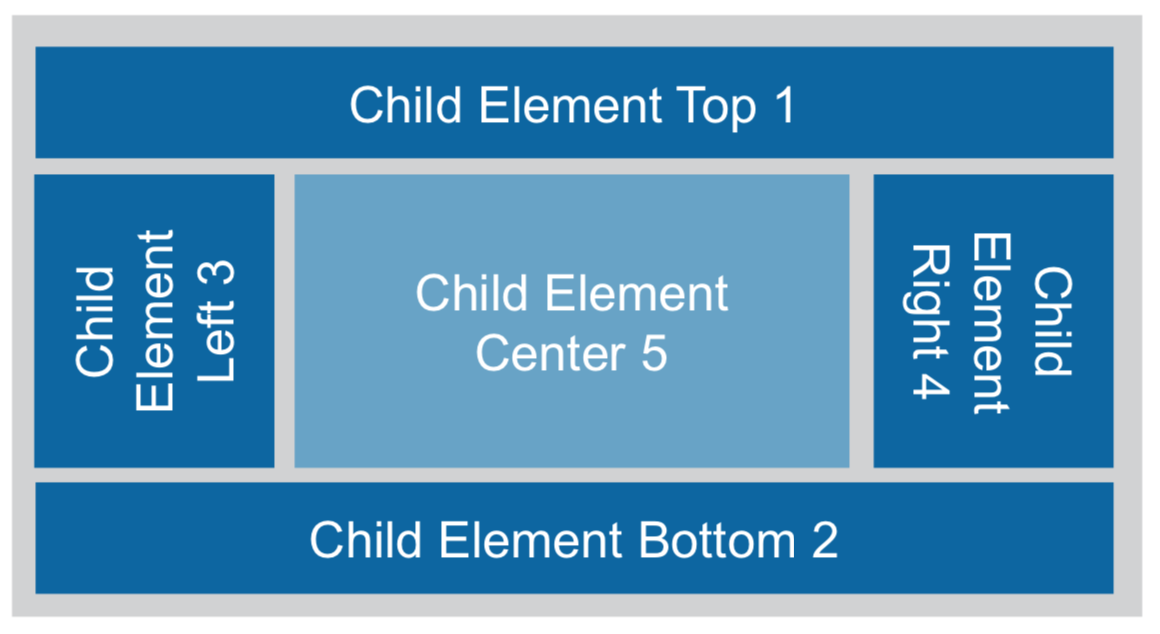
\includegraphics[scale=0.35]{DockPanel.png}
\paragraph{Grid} Im Grid können Child Elemente einer Zelle darin zugeordnet werden. Die Zeilen und Spalten müssen explizit angegeben werden

Sie haben jeweils ein optionales \code{Height}/\code{Width}-Attribut. Der Default-Wert ist \code{Auto}, was bedeutet dass nur der benötigte Platz benutzt werden soll. Zusätzlich zu den normalen Grössenangabewerten gibt es noch die Stern-Definition. Damit kann eine Art Gewicht vergeben werden, und die Elemente füllen den vorhandenen Platz aus. Fürs reine Füllen gibt es die Variante 1 Stern (\code{Height="*"}), fürs Gewicht z.B. die Variante 3 Stern (\code{Height="3*"}).
\begin{lstlisting}[language=xml, caption="3 x 3 Grid"]
<Grid>
    <Grid.ColumnDefinitions>
        <ColumnDefinition></ColumnDefinition>
        <ColumnDefinition></ColumnDefinition>
        <ColumnDefinition></ColumnDefinition>
    </Grid.ColumnDefinitions>
    <Grid.RowDefinitions>
        <RowDefinition></RowDefinition>
        <RowDefinition></RowDefinition>
        <RowDefinition></RowDefinition>
    </Grid.RowDefinitions>
</Grid>
\end{lstlisting}
Auf den einzelnen Definitions kann man \code{Width} und \code{Height} definieren (sowie Min/Max etc.). Ebenfalls ist es mit \code{RowSpan} bzw. \code{ColumnSpan} möglich, Elemente über mehrere Zellen/Spalten zu strecken. \\
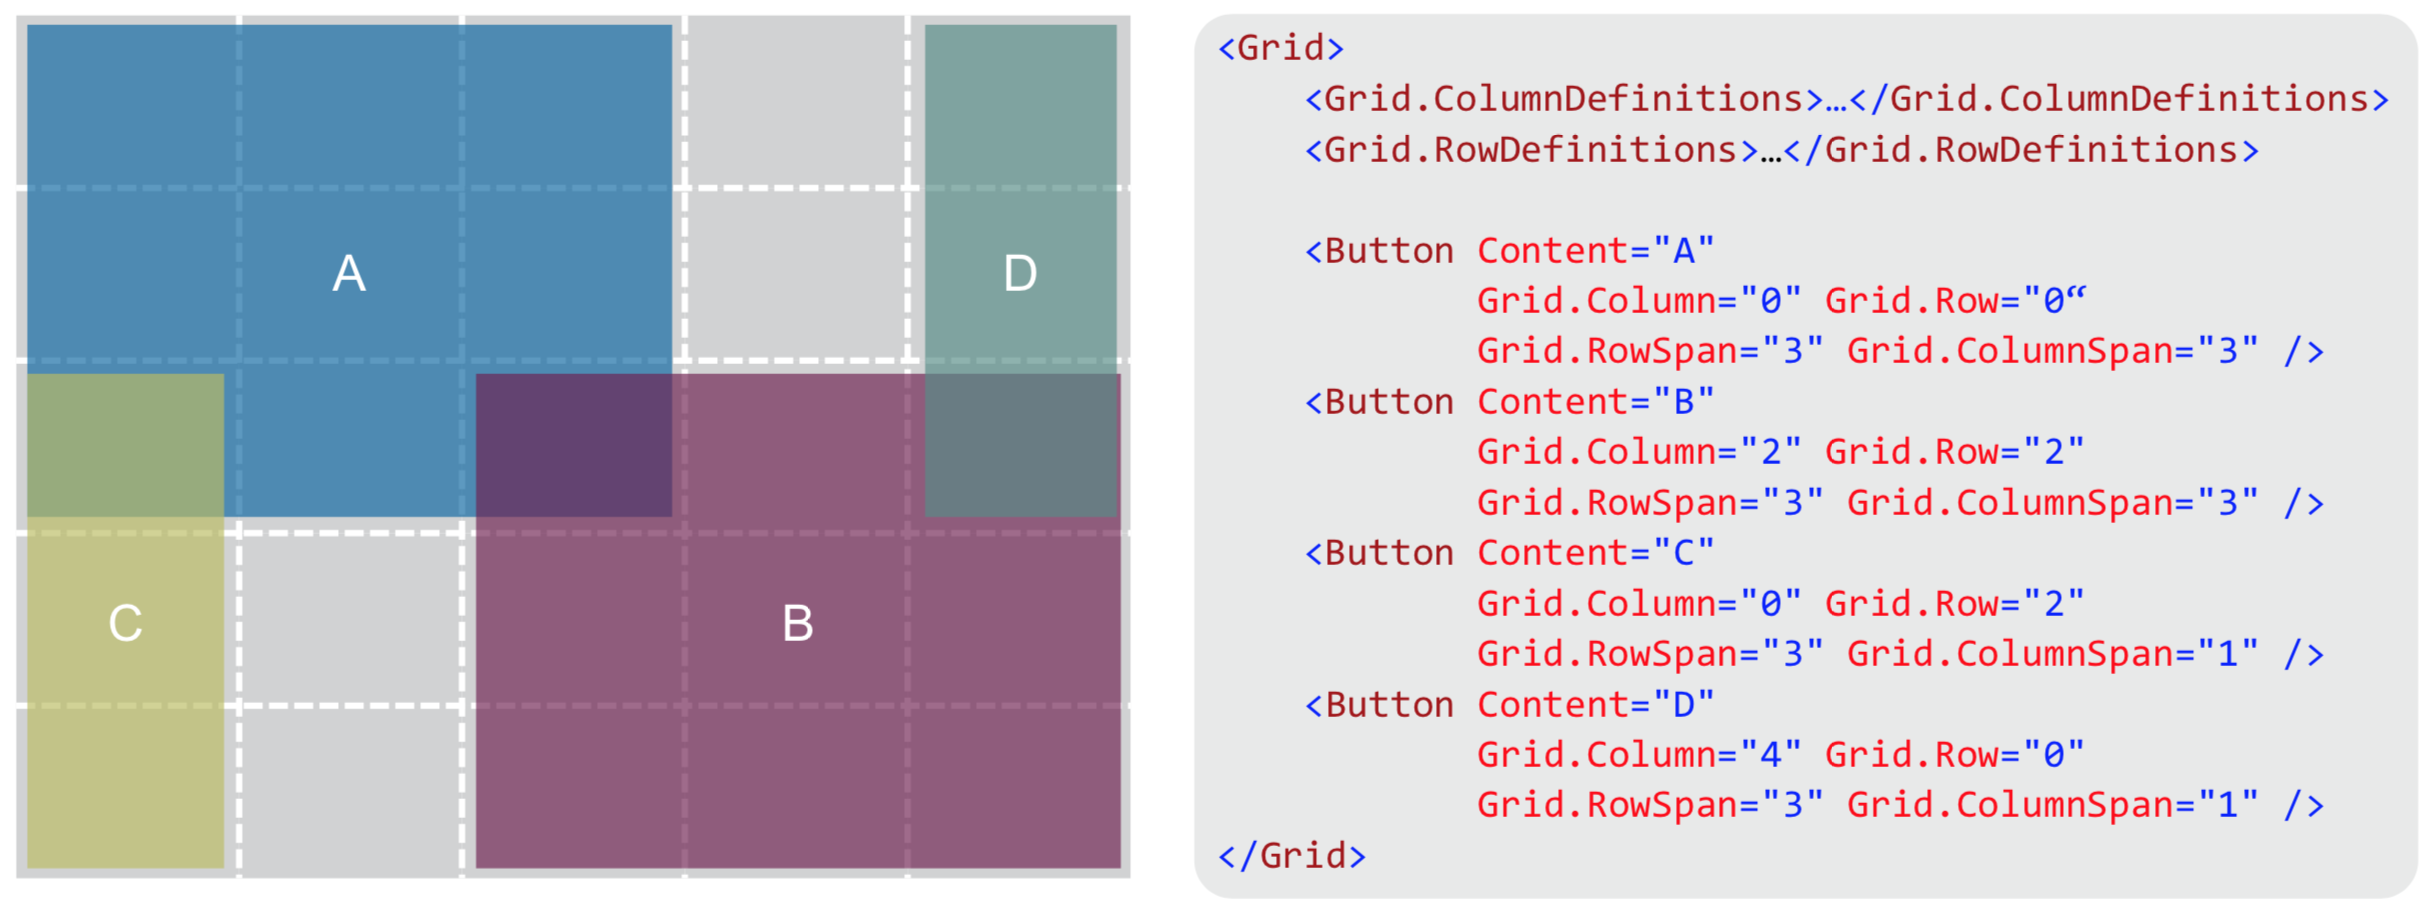
\includegraphics[scale=0.35]{Grid.png}
\begin{lstlisting}[language=xml]
<Grid>
    <Grid.ColumnDefinitions>...</Grid.ColumnDefinitions>
    <Grid.RowDefinitions>...</Grid.RowDefinitions>
    <Button Content="A"
        Grid.Column="0" Grid.Row="0"
        Grid.RowSpan="3" Grid.ColumnSpan="3" />
    <Button Content="B"
        Grid.Column="2" Grid.Row="2"
        Grid.RowSpan="3" Grid.ColumnSpan="3" />
    <Button Content="C"
        Grid.Column="0" Grid.Row="2"
        Grid.RowSpan="3" Grid.ColumnSpan="1" />
    <Button Content="D"
        Grid.Column="4" Grid.Row="0"
        Grid.RowSpan="3" Grid.ColumnSpan="1" />
</Grid>
\end{lstlisting}
\textbf{Spezialfall} Bei einem 1 x 1 Grid werden die Elemente in der Zelle gestapelt und man kann mit Alignments und Margin ein flexibles Layout erstellen. Mit dem GridSplitter kann man die Spalten und Zellengössen anpassen. Mit der SharedSizeGroup können mehrere Spalten/Zeilen verknüpft werden um eine einheitliche Breite/Höhe festzulegen.
\paragraph{Canvas} In einem Canvas Control haben alle Elemente eine absoulte Positionierung und es gibt keine Layout Logik. Die Position innerhalb des Canvas kann mittels \textbf{Attached Properties} festgelegt werden:
\begin{itemize}
\item \code{Canvas.Left}: Abstand vom linken Rand
\item \code{Canvas.Top}: Abstand vom oberen Rand
\item \code{Canvas.Right}: Abstand vom rechten Rand
\item \code{Canvas.Bottom}: Abstand zum unteren Rand
\item \code{Canvas.ZIndex}: Z-Position (Ebene) im Canvas
\end{itemize}
In Verbindung mit \code{Shapes} ist ein Canvas Control gut zum "{}programmierten Zeichnen"{} geeignet.
\begin{lstlisting}[language=xml]
<Canvas>
    <Rectangle
        Canvas.Left="80" Canvas.Top="60"
        Width="128" Height="80"
        Fill="#006aa6" />
    <Ellipse
        Canvas.Left="260" Canvas.Top="160"
        Width="120" Height="120"
        Fill="#6E1C50" />
    <Path
        Canvas.Left="120" Canvas.Top="64"
        Width="260" Height="200"
        Stroke="DarkGray" Stretch="Fill"
        Data="M1,0 L0,1"/>
</Canvas>
\end{lstlisting}
\paragraph{Shapes} Die Shapes Klasse beinhaltet \code{Ellipse}, \code{Polygon}, \code{Line}, \code{Polyline}, \code{Path} und \code{Rectangle}. Alle Shapes haben folgende Attribute:
\begin{itemize}
\item \textbf{Fill:} Brush für die Füllung
\item \textbf{Stroke:} Pen für Rahmen/Pinselstrich
\item \textbf{StrokeThickness:} Breite des Rahmens/Pinselstrichs
\item \textbf{StrokeDasharray:} Muster für gestrichelte Linien
    \subitem \textbf{"{}2 1"{}} ist das Verhätniss zwischen Linie/Lücke immer 2:1
    \subitem \textbf{"{}2 1 4 1"{}} ist das Verhältniss zuerst 2:1, dann 4:1 dann 2:1 etc.
\item \textbf{StrokeLineJoine:} Art des Übergangs bei Ecken
    \subitem \textbf{Miter:} Spitzer Rand
    \subitem \textbf{Bevel:} Abgeschnittener Rand
    \subitem  \textbf{Round:} Abgerundeter Rand
\end{itemize}
\paragraph{ViewBox} Skaliert, mittels Transformation, ein einzelnes Child Control um den Verfügbaren Platz auszunutzen. Das Attribut \code{Strech} kann verwendet werden um zu definieren wie das Control skaliert werden soll. Valid sind: \code{None} (keine Skalierung), \code{Uniform} (Vergrössern bis es ins Controll passt), \code{Fill} (Strecken, dass kompletter Platz verwendet wird), \code{UniformToFill} (Vergrössern und Strecken, dass Proportionen erhalten bleiben, aber ganzes Control ausgefüllt wird. Bei Übergrösse wird das Alignment berücksichtigt.
\paragraph{Border} Die Border zeichnet lediglich ein Rahmen um ein Child Control. Es kann mit Panels kombiniert werden.
\begin{lstlisting}[language=xml]
<Border Background="GhostWhite" CornerRadius="8,0,8,0"
        BorderBrush="#ddd" BorderThickness="1"
        Margin="10"
        Padding="10">
    <StackPanel Orientation="Vertical">
        <Button Margin="0,0,0,5" Content="Dock Sample 1" />
        <Button Margin="0,0,0,5" Content="Dock Sample 2" />
        <Button Margin="0,0,0,5" Content="Grid Sample 1" />
        <Button Margin="0,0,0,5" Content="Grid Sample 2" />
        <Button Margin="0,0,0,5" Content="Grid Sample 3" />
        <Button Margin="0,0,0,5" Content="Canvas Sample 3" />
    </StackPanel>
</Border>
\end{lstlisting}
\subsection{Input Controls}
\paragraph{Texteingabe} Für die Texteingabe gibt es die \code{TextBox} (Normalen Text Input, mit Option für mehrzeilige Eingabe), \code{RichTextBox} (Text Input mit Formatierung) und die \code{PasswordBox}.
\paragraph{Buttons} Es gibt verschiedene Arten von Buttons: \code{Button}, \code{RepeatButton} (Löst Click-Event wiederholt aus, bis Button losgelassen wird), \code{ToggleButton} (hat zwei Zustände), \code{RadioButton}, \code{CheckBox}.
\subsection{List Control}
\paragraph{Listen} Es gibt verschiedene Listen in WPF. Die \code{ListBox} ist eine komplett sichtbare (scrollable) Liste mit Daten. Diese Einträge können auch Formatierungen beinhalten.
\begin{lstlisting}
<ListBox SelectedIndex="1" SelectionMode="Multiple">
    <ListBoxItem>Erster Eintrag</ListBoxItem>
    <ListBoxItem>Zweiter Eintrag</ListBoxItem>
    <StackPanel Orientation="Horizontal">
        <Rectangle Width="10" Height="10" Fill="Blue" />
        <TextBlock Margin="10,0">Dritter Eintrag</TextBlock>
    </StackPanel>
</ListBox>
\end{lstlisting}

\subsection{ItemTemplate}
In einer ListBox festlegen, wie die Items angezeigt werden sollen
\begin{lstlisting}
<DataTemplate x:Key="myTaskTemplate" DataType="local:Task">
    <DockPanel HorizontalAlignment="Stretch">
        <TextBlock Text="{Binding TaskName}" />
        <TextBlock Text="{Binding Description}" />
        <TextBlock Text="{Binding Priority}" />
    </DockPanel>
</DataTemplate>

<ListBox ItemSource="{Binding Source={Static Resource myTodoList}}"
    ItemTemplate="{StaticResource myTaskTemplate}" />
\end{lstlisting}

Die ComboBox ist eine normale DropDown Liste. Sie kann editierbar gemacht werden, mit \code{IsEditable} bzw. \code{IsReadOnly}.
\begin{lstlisting}[language=xml]
<ComboBox SelectedIndex="0">
    <ComboBoxItem>Erster Eintrag</ComboBoxItem>
    <ComboBoxItem>Zweiter Eintrag</ComboBoxItem>
</ComboBox>
\end{lstlisting}
Eine \code{ListView} ist ein Read-Only DataGrid, eine generalisierte Anzeige einer Liste (Explorer Ansichten).\\
Eine \code{TreeView} ist eine hierarchische Anzeige von Daten in einer Baumstruktur (Windows Explorer Pfad Baum).
\subsection{Beschriftungen} 
\paragraph{TextBlock} Dies ist eine einfache Textanzeige, kein vollwertiges Control. Es kann auch als einfaches "{}Spacer"{} Element gebraucht werden.
\paragraph{Label} Ein Label kann mittels Keyboard Shortcuts aufgerufen werden (vollwertiges Control). Es kann nicht nur Text anzeigen, sondern auch Layouts beinhalten und das Aussehen kann mittels Templates gestaltet werden.
\paragraph{ToolTip} Das ToolTip kann kontextbezongene Infos bei einem Mouse-Over anzeigen, es kann ebenfalls ein beliebiges Layout beinhalten. Bei deaktivierten Controls muss die Property \code{ToolTipService.ShowOnDisabled} gesetzt werden, wenn ToolTip trotzdem erscheinen soll.
%TODO: W09 - Layout und Controls, Folie 49, ToolTip Grafik
\begin{lstlisting}
<Button.ToolTip>
    <StackPanel>
        <TextBlock Text="Submit Button"
            FontWeight="Bold" />
        <TextBlock Text="Submits ..." />
    </StackPanel>
</Button.ToolTip>
\end{lstlisting}
\subsection{Wertebereiche}
\paragraph{Progress Bar} wird verwendet um den Benutzer auf eine lange andauernde Operation hinzuweisen. Mit Container Controls kann dieser beliebig dekoriert werden. 
\begin{lstlisting}[language=xml]
<ProgressBar Minimum="0" Maximum="100" Value="75" />
\end{lstlisting}
\paragraph{Slider} Der Slider gibt eine Auswahl aus einem vorgegeben Wertebereich zurück
\begin{lstlisting}[language=xml]
<Slider Maximum="100" Value="75" TickFrequency="10" TickPlacement="BottomRight" />
\end{lstlisting}
\subsection{Organisation}
\paragraph{GroupBox} gruppiert visuell zusammengehörende Controls
\begin{lstlisting}[language=xml]
<GroupBox Header="Mouse Handedness">
    <StackPanel>
        <RadioButton Content="Left-Handed" />
        <RadioButton Content="Right-Handed"
            IsChecked="True"/>
    </StackPanel>
</GroupBox>
\end{lstlisting}
\paragraph{Expander} ermöglicht das Ein und Ausblenden von Infos bei Bedarf. Er wird oft für Zusatzinformationen gebraucht.
\begin{lstlisting}[language=xml]
<Expander>
    <Expander.Header>More info</Expander.Header>
    <TextBlock TextWrapping="Wrap" Text="Drag ..." />
</Expander>
\end{lstlisting}
\paragraph{TabControl} teilt das UI in mehrere Seiten auf. Jedes \code{TabItem} enthält ein eigenes Layout. Das Header Attribut kann mit beliebigem Layout gefüllt werden.
\begin{lstlisting}[language=xml]
<TabControl>
    <TabItem Header="1 - Intro">
        <Grid Margin="10">
        ...
        </Grid>
    </TabItem>
    <TabItem Header="2 - Daten" />
    <TabItem Header="3 - Optionen" />
    <TabItem>
        <TabItem.Header>
            <StackPanel Orientation="Horizontal">
                <Grid>
                    <Ellipse Fill="Silver" Width="16"
                        Height="16" />
                    <Label Content="4" FontSize="10"
                        Foreground="White" />
                </Grid>
            <TextBlock Text="Review" />
            </StackPanel>
        </TabItem.Header>
    </TabItem>
</TabControl>
\end{lstlisting}
\paragraph{Eigene Controls} Es gibt zwei Arten von Controls. Das \code{UserControl} welches als \textbf{Komposition} implementiert wird. Es ist eine Wiederverwendbare Zusammenstellung mehrer COntrols als Gruppe und besteht aus einem XAML und Code-Behind. Es kann nicht mit Styles/Templates umgehen.\\
Das \code{CustomControl} ist eine Ableitung der zu verändernden Klasse. Es erweitert ein bestehendes Control um neue Funktionen. Es besteht aus einem Code-File und ggf. aus einem Standart-Style. Es kann mit Styles/Templates umgehen.



\subsection{Data Grid}

\begin{lstlisting}[language=xml]
<DataGrid ItemsSource="{Binding Customers}"
    AutoGenerateColumns="False" >
  <DataGrid.Columns>
    <DataGridTextColumn Header="First Name" 
        Binding="{Binding FirstName}" />
  </DataGrid.Columns>
  <DataGrid.Columns>
    <DataGridTemplateColumn Header="Image" Width="SizeToCells" 
        IsReadOnly="True">
      <DataGridTemplateColumn.CellTemplate>
        <DataTemplate>
          <Image Source="{Binding Image}" />
        </DataTemplate>
      </DataGridTemplateColumn.CellTemplate>
    </DataGridTemplateColumn>
  </DataGrid.Columns>
</DataGrid>
\end{lstlisting}

\subsection{Package URI}
\begin{itemize}
    \item \code{siteOfOrigin}: relativ zum aktuellen Ordner
    \item \code{application}: relativ zum Assembly
\end{itemize}


